\section{Method}

\subsection{Outline of the Proposed Method}

Our approach relies on the well-known observation that the greater the similarity between two projections, the more likely they originated from two 3D particles that adopted close orientations in the ice layer prior to imaging\footnote{Up to some possible intrinsic symmetries of the objects, which are discussed later.}. This principle guides a number of applications in SPA, including that of projection matching~\cite{penczek1994ribosome}.

Taking this line of thought further, we train a function---parametrized as a neural network---to predict the relative orientation between two projections based on their similarity. To make such training possible, we capitalize on our ability to model the cryo-EM imaging procedure to generate a large, representative synthetic dataset using publicly available 3D atomic models.

Using this trained distance function, we can estimate the relative orientations between pairs of projections in any real dataset. Our postulate is that we can then recover, from these estimated relative orientations, the orientations themselves through an appropriate minimization scheme. This two-steps pipeline is illustrated in Figure~\ref{fig:overview-pipeline}. \\

% ---
\begin{figure}[h!]
    \center
    \fbox{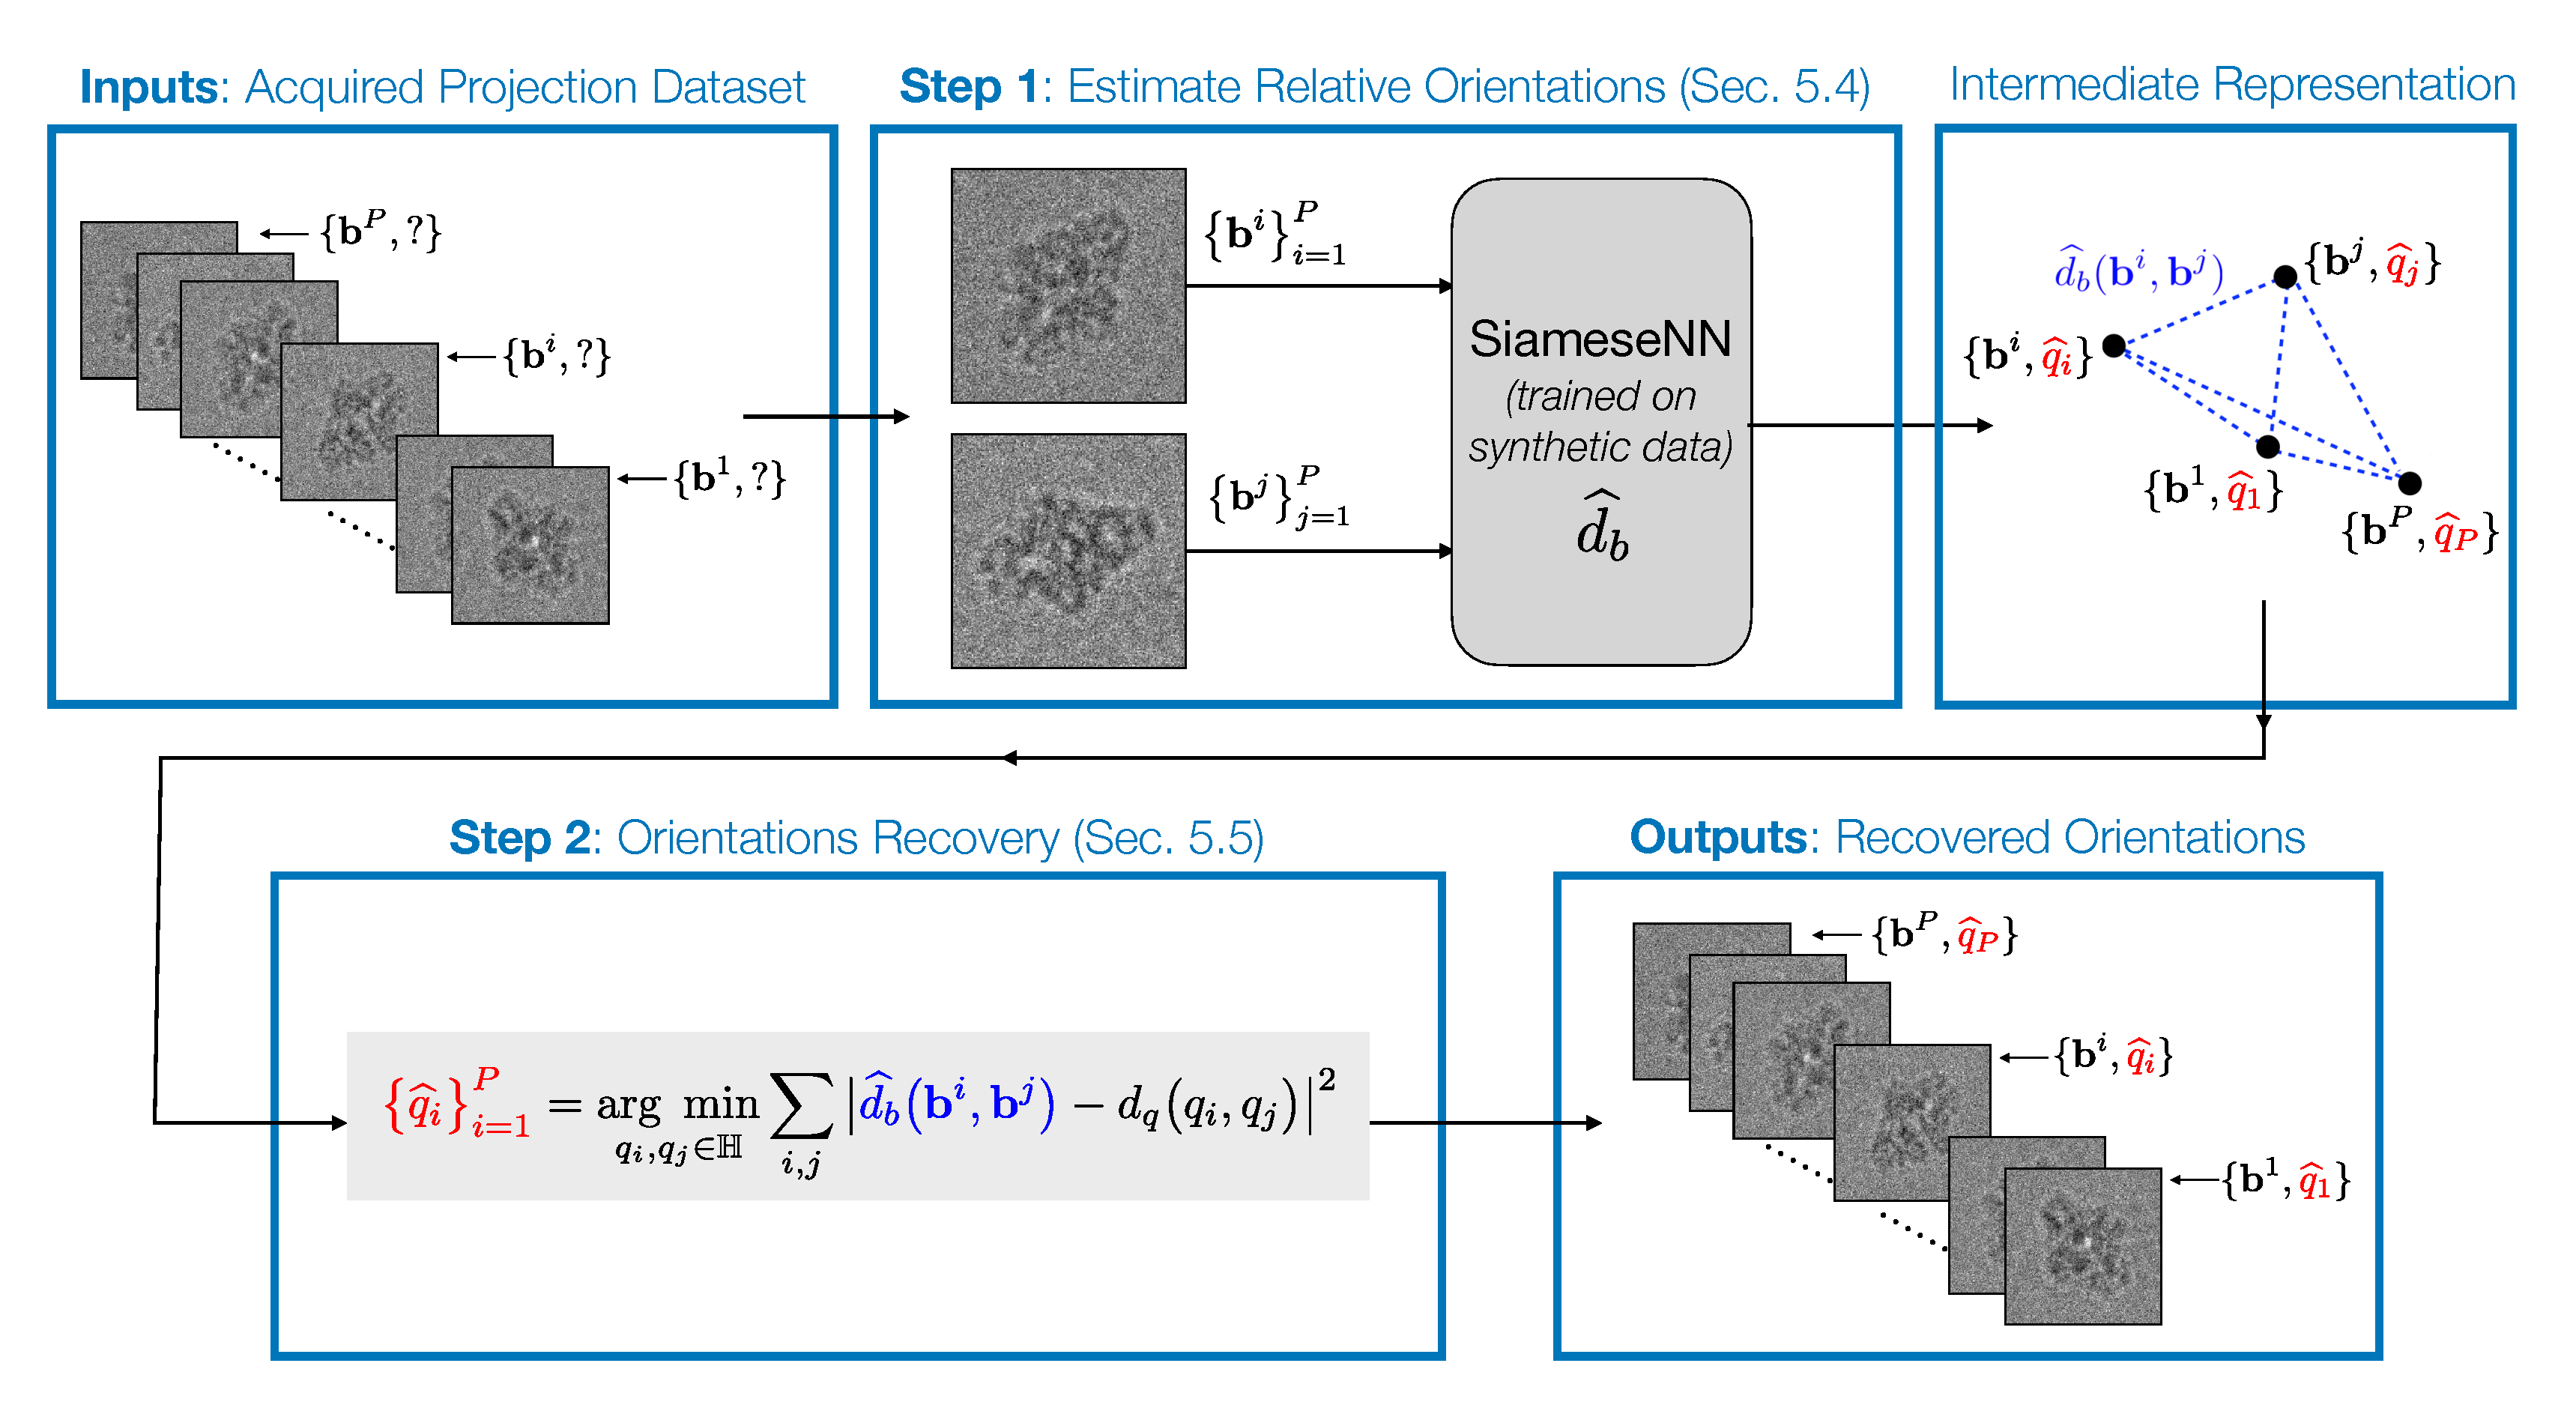
\includegraphics[width=\textwidth]{pipeline-overview.pdf}}
    \caption{Overview of the proposed two-steps method: 1) estimate the relative orientations between projection pairs through a learned distance $\widehat{d}_b$, and 2) recover the orientations from the estimated relative orientations. We denote a $p$th projection by $\mathbf{b}^p$ and its orientation by $q_p$. The geodesic distance between two orientations is denoted by $d_q$.}
    \label{fig:overview-pipeline}
\end{figure}
% ---

The task of recovering points based on their relative distances has been extensively studied in the literature, mostly within the framework of dimensionality reduction and primarily for the case of \textit{Euclidean} embedding spaces\footnote{An ``embedding space'' corresponds to the (often lower-dimensional) space in which data is embedded, \textit{i.e.}, mapped to in such a way that the relative distances between its points are preserved as much as possible.}~\cite{belkin2003laplacian,kruskal1978multidimensional, maaten2008visualizing, mcinnes2018umap,dokmanic2015euclidean} . In that respect, the short example given by Dokmanic \textit{et al.} in~\cite{dokmanic2015euclidean} efficiently illustrates the philosophy behind such methods (see the ``An Analogy'' box). \\

% ---------------------------------------------------
\setlength{\fboxsep}{1em}\noindent\fbox{\parbox{0.95\textwidth}{%
\textbf{An Analogy: Mapping the Position of Swiss Cities with a Train Timetable~\cite{dokmanic2015euclidean}} \\

% ---
\begin{wrapfigure}{r}{0.45\textwidth}
  \begin{center}
    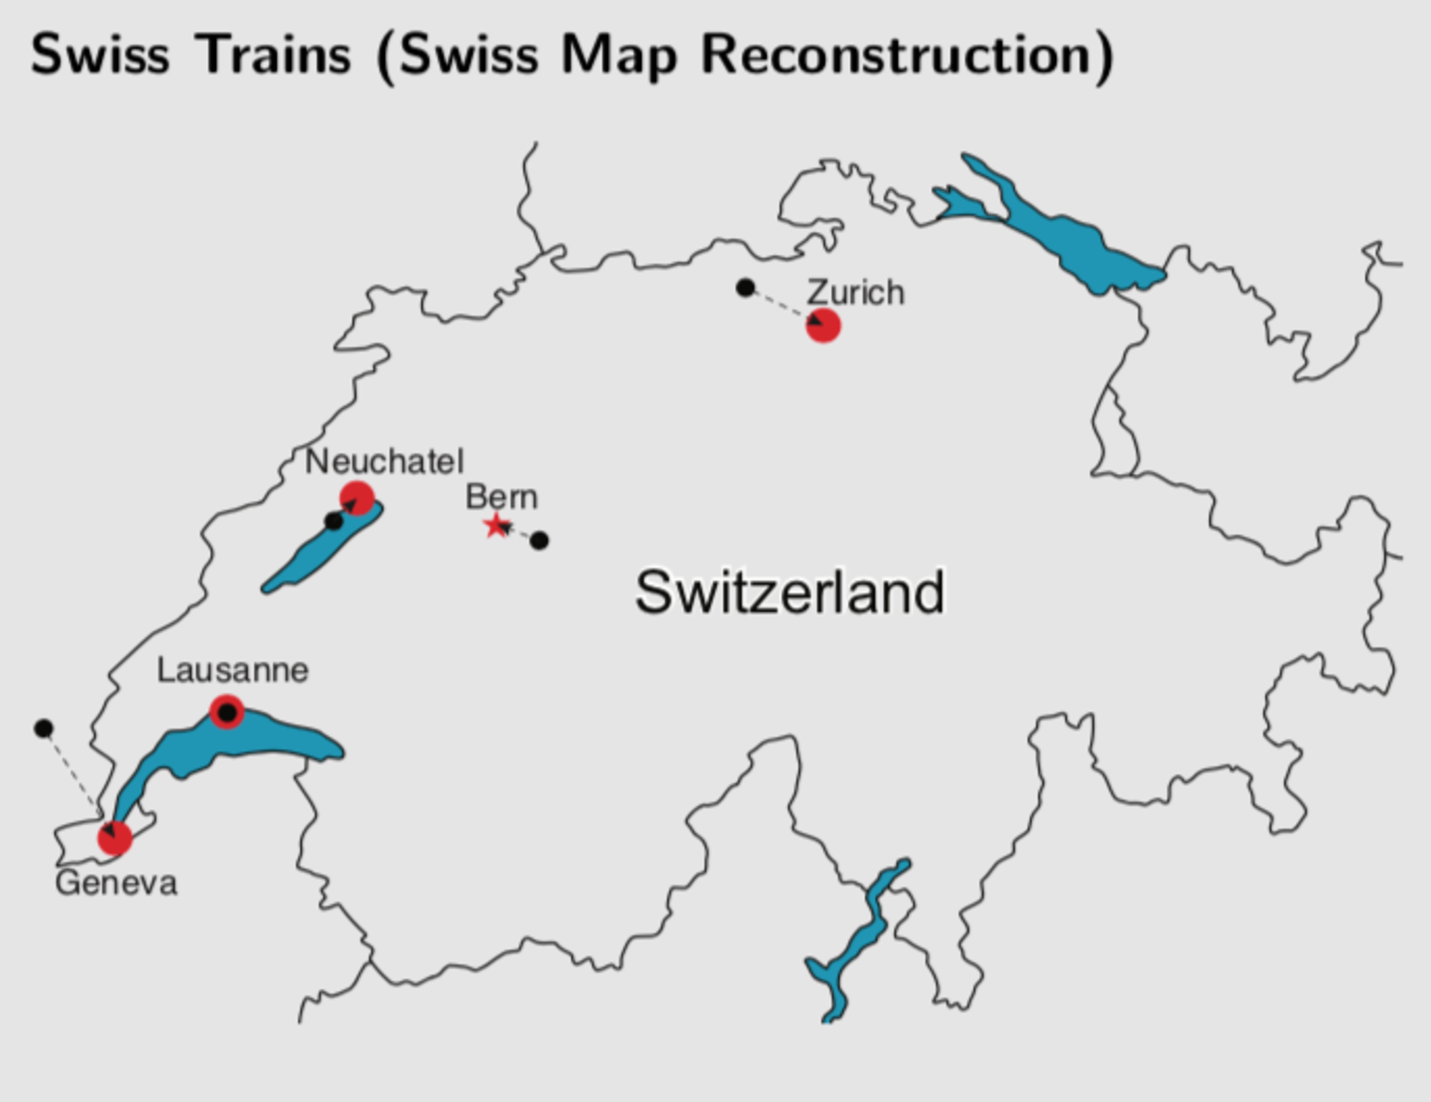
\includegraphics[width=0.4\textwidth]{swissEDM.pdf}
  \end{center}
  \caption{\footnotesize Image adapted from~\cite{dokmanic2015euclidean}. The red signs indicate the correct city locations. The black dots denote the recovered city locations.}
\end{wrapfigure}
% ---
\small
In this toy problem, the authors aim at estimating the position of five cities on the Swiss map based not on the spatial distances between them, but on the time it takes to travel by train between them. Those time data (in minutes) are collected in the following timetable: \vspace{0.25cm}

%---
{\footnotesize\begin{blockarray}{cccccc}
& \text{L} & \text{G} & \text{Z} & \text{N} & \text{B} \\
\begin{block}{l(ccccc)}
  \text{Lausanne}  & 0   & 33  & 128 & 40 & 66 \\
  \text{Geneva}    & 33  & 0   & 158 & 64 & 101 \\
  \text{Zürich}    & 128 & 158 & 0   & 88 & 56 \\
  \text{Neuchâtel} & 40  & 64  & 88  & 0  & 34 \\
  \text{Bern}     & 66  & 101 & 56  & 34 & 0 \\
\end{block}\end{blockarray}.} \\

%---
Remarkably, even though these time data only roughly correlate with the physical distances between the cities, one can still obtain a remarkably good estimate of their positions on the Swiss map (up to some symmetries of the embedding space) using a multidimensional scaling algorithm.
}}\normalsize \\
% ---------------------------------------------------

This example, if rather simple, nevertheless underlines well the key ingredients of methods that aim at retrieving points from distances that may not be directly measurable:
%---
\begin{enumerate}
    \item \textit{An appropriate proxy for the ``real'' distance}. In the above example, the proxy for the spatial distance between two cities is the time taken to travel by train between them. In our case, we shall consider the similarity between two projections to be a good proxy for their relative orientation.
    %
    \item \textit{A sufficiently rich collection of proxy distance data}. In this example, these data are provided by the (complete) train timetable. In our approach, we shall estimate the relative orientations between numerous pairs of projections based on the aforementioned proxy distance.
    %
    \item \textit{An efficient recovery scheme}. In~\cite{dokmanic2015euclidean}, the embedding space being Euclidean, the theoretical framework of the Euclidean distance matrices (EDMs) guarantees that one can retrieve the desired points from the collected distances. In our case, as we shall shortly explain, we aim to embed the estimated relative orientations on $\SOThree$, the space of 3D rotations. Unfortunately, the extension of the EDM theory to such manifold is all but straightforward.
\end{enumerate}
%---

There is no simple way to ``handcraft'' a proxy distance that would robustly predict the similarity between two projections. Hence, we resort to \textit{learning} this distance function by parametrizing it as a neural network and capitalizing on 1) the public availability of large datasets of 3D atomic models\footnote{\texttt{https://www.ebi.ac.uk/pdbe/emdb}}, and 2) our ability to model the cryo-EM imaging process. This is the topic of Section~\ref{sec:estimating-relative-orientations}.

Equipped with this learned distance, the idea is then to apply the aforementioned two-steps method (see Figure~\ref{fig:overview-pipeline}) for any projection dataset. As we just mentioned, we cannot rely on the theoretical framework of EDMs since our embedding space is non-Euclidean. Despite this lack of theoretical guarantees, we are able to appropriately minimize our objective function using a gradient-based algorithm, as we experimentally demonstrate in Section~\ref{sec:orientation-recovery}.

As a preamble, we discuss the need for a representation of orientations in $\SOThree$ that relies on unit quaternions.

\subsection{Unit Quaternions and the Geodesic Distance}
\label{sec:quaternions}

As mentioned, our objective is to recover unknown 3D orientations by embedding their estimated relative distances on the $\SOThree$ space. As we shall explain in the next sections, this embedding requires the efficient computation of the relative distance between two rotations $\mathbf{R}_1, \mathbf{R}_2 \in\SOThree$, which corresponds to the rotation $\mathbf{R}_*\in\SOThree$ such that $\mathbf{R}_1=\mathbf{R}_*\mathbf{R}_2$.

It is standard in SPA to work with Euler angles to describe the orientation of a 3D object in the electron microscope. More precisely, one relies on the parametrization $\bth=(\theta_1,\theta_2,\theta_3)\in\Omega_\bth$, with $\Omega_\bth=[0;2\pi)\times [0;\pi] \times [0;2\pi)$, to encode the 3D rotation that relates the object coordinate system to the projection coordinate system.

Unfortunately, the relative distance between two rotations $\mathbf{R}(\bth_1)$, $\mathbf{R}(\bth_2)$, parametrized by Euler angles cannot be directly computed from $\bth_1$, $\bth_2$. It requires the computation of the rotation matrices, which is computationally inefficient\footnote{Another technical challenge with Euler angles is that they suffer from the so-called gimbal lock problem, which arises when $\theta_2=0$ and restricts the number of rotational degrees of freedom to one even though $\theta_1$ and $\theta_3$ have not yet been fixed~\cite{koks2006explorations}.}. Hence, we resort to a more convenient representation of 3D rotations that relies on unit quaternions.

The algebra of quaternions was introduced in the mid-nineteenth century by Hamilton~\cite{rosenfeld_history_1988}. A quaternion $q\in\mathbb{H}$ takes the form
%---
\begin{equation}
    \label{eq:quaternion-definition}
    q =  a\boldsymbol{1} + b\boldsymbol{i} + c\boldsymbol{j} + d\boldsymbol{k},
    \end{equation}
%---
where $(a,b,c,d)\in\mathbb{R}^4$, and $\boldsymbol{1}$, $\boldsymbol{i}$, $\boldsymbol{j}$, and $\boldsymbol{k}$ are the fundamental quaternion units
%---
\begin{equation}
    \label{eq:quaternion-units}
    \boldsymbol{1} = \begin{pmatrix} 1 & 0 \\ 0 & 1 \end{pmatrix}, \quad
    \boldsymbol{i} = \begin{pmatrix} i & 0 \\ 0 & -i \end{pmatrix}, \quad
    \boldsymbol{j} = \begin{pmatrix} 0 & 1 \\ -1 & 0 \end{pmatrix}, \quad
    \boldsymbol{k} = \begin{pmatrix} 0 & i \\ i & 0 \end{pmatrix},
\end{equation}
%---
with $i$ the imaginary unit. Any quaternion $q$ can thus be represented by its set of coefficients $(a,b,c,d)\in\mathbb{R}^4$. The algebra $\mathbb{H}$ is similar to the algebra of complex numbers $\mathbb{C}$, with the exception of the multiplication operation being noncommutative.

In this work, we restrict our interest to unit quaternions $q\in\mathbb{U}$, with  $\mathbb{U}=\big\{q\in\mathbb{H} \; \, | \; \,\lvert q \rvert =1\big\}$, which identify the $\mathbb{S}^3$ hypersphere in  $\mathbb{R}^4$. Unit quaternions concisely and elegantly represent the elements of the $\SOThree$ group. More precisely, a unit quaternion $q\in\mathbb{U}$ parametrizes a rotation $\mathbf{R}\in\SOThree$ through
% ---
\begin{equation}
    \mathbf{R}(q) =\begin{pmatrix}
    a^2+b^2-c^2-d^2 & 2bc-ad & 2bd+2ac  \\
    2bc+2ad & a^2-b^2+c^2d^2 & 2cd-2ab \\
    2bd-2ac & 2cd+2ab & a^2-b^2-c^2+d^2
    \end{pmatrix}.
    \label{eq:quaternion-rotation-matrix}
\end{equation}
% ---

The geodesic distance $d_q:\mathbb{U}\times\mathbb{U}\rightarrow [0,\pi]$ between two unit quaternions $q_i, q_j\in\mathbb{H}$ is then defined as
% ---
\begin{equation}
    \label{eq:geodesic distance}
    d_q(q_i,q_j)=2\arccos\big(|\langle q_i, q_j \rangle|\big),
\end{equation}
% ---
with the inner product between quaternions given by
% ---
\begin{equation}
    \label{eq:inner-product-quaternions}
    \langle q_i, q_j \rangle = a_ia_j+b_ib_j+c_ic_j+d_id_j.
\end{equation}
% ---
The distance~\eqref{eq:geodesic distance} is the shortest distance between $q_i$ and $q_j$ on the surface of $\mathbb{S}^3$.

As $\mathbb{S}^3$ is isomorphic to the universal cover of $\SOThree$, the geodesic distance corresponds to the magnitude of the relative orientation $\mathbf{R}_*$ between $\mathbf{R}(q_i)$ and $\mathbf{R}(q_j)$ in $\SOThree$~\cite{huynh2009metrics}. In other words, the relative distance between two rotations encoded by unit quaternions can be efficiently computed from the unit quaternions themselves through~\eqref{eq:geodesic distance}, which is of key practical importance for this work.

For the sake of conciseness, we shall use the term ``with orientation~$q$'' to refer to 2D/3D objects considered in an imaging geometry parametrized by $q$.

\subsection{Estimating Relative Orientations from Projections}
\label{sec:estimating-relative-orientations}

Equipped with the geodesic distance $d_q$, our goal is now to find a ``projection distance'' $d_b$ that is a good predictor of $d_q$. Before discussing the different options, we briefly describe the synthetic datasets used in this work.

% -------------------------------
\subsubsection{Experimental Dataset}
\label{subsec:datasets}

We consider two proteins as ground truths: the $\beta$-galactosidase, a protein with a dihedral (D2) symmetry, and the lambda excision HJ intermediate (HJI), an asymmetric protein. Their deposited PDB atomic models are 5a5a ~\cite{bartesaghi2015betagal} and 5j0n~\cite{laxmikanthan2016structure}, respectively. For each atomic model, we generate the ground truth by fitting a 5\AA\ density map in Chimera~\cite{pettersen2004ucsf}. We thus obtain a volume of size $(117\times 117\times 117)$ for the $\beta$-galactosidase, and a volume of size $(275\times 275\times 275)$ for the HJI.

From these ground truths, we generate $5,000$ synthetic projections of size $(117\times 117)$ and $(275\times 275)$, respectively, using the ASTRA projector~\cite{van2015astra}. The projection orientations are sampled from a uniform distribution over half the $\SOThree$ space, which suffices to generate all the possible projections of a volume. For the sake of simplicity, the projections are currently kept unblurred and noiseless. Whenever training neural networks, we split the datasets into a distinct training set (50\%), validation set (22\%), and testing set (33\%), to ensure that the results can generalize to unseen projections. The complete pipeline is implemented in Tensorflow~\cite{abadi2016tensorflow}.


% -------------------------------
\subsubsection{Baseline Test with the Euclidean Distance}

As a baseline, we first evaluate the suitability of the Euclidean distance as a projection distance $d_b$ to predict $d_q$. For the two aforementioned datasets, we randomly select $1,000$ pairs of projections. For each pair, we compute the Euclidean distance between the projections $d_b(\mathbf{b}^i,\mathbf{b}^j)=\lVert\mathbf{b}^i-\mathbf{b}^j\rVert_2$ and their relative orientation $d_p(q_i,q_j)$ through~\eqref{eq:geodesic distance}. We then report the $(d_q,d_b)$ relationship for all pairs in Figure~\ref{fig:euclidean-not-robust}, for both the asymmetric protein (left) and the symmetric one (right).


Two principal observations can be made from this experiment. First, as suspected, the Euclidean distance between projections fails to be a consistent predictor of their relative orientation distance, even in the simple imaging conditions considered here (no noise and no effect of the PSF). In particular, the larger the relative distance $d_q$, the poorer the predictive ability of the Euclidean distance as $d_b$. The other interesting observation is that the intrinsic symmetry of the $\beta$-galactosidase protein (5a1a) appears in its $(d_q,d_b)$ plot.

%-----
\begin{figure}[t]
    \centering
    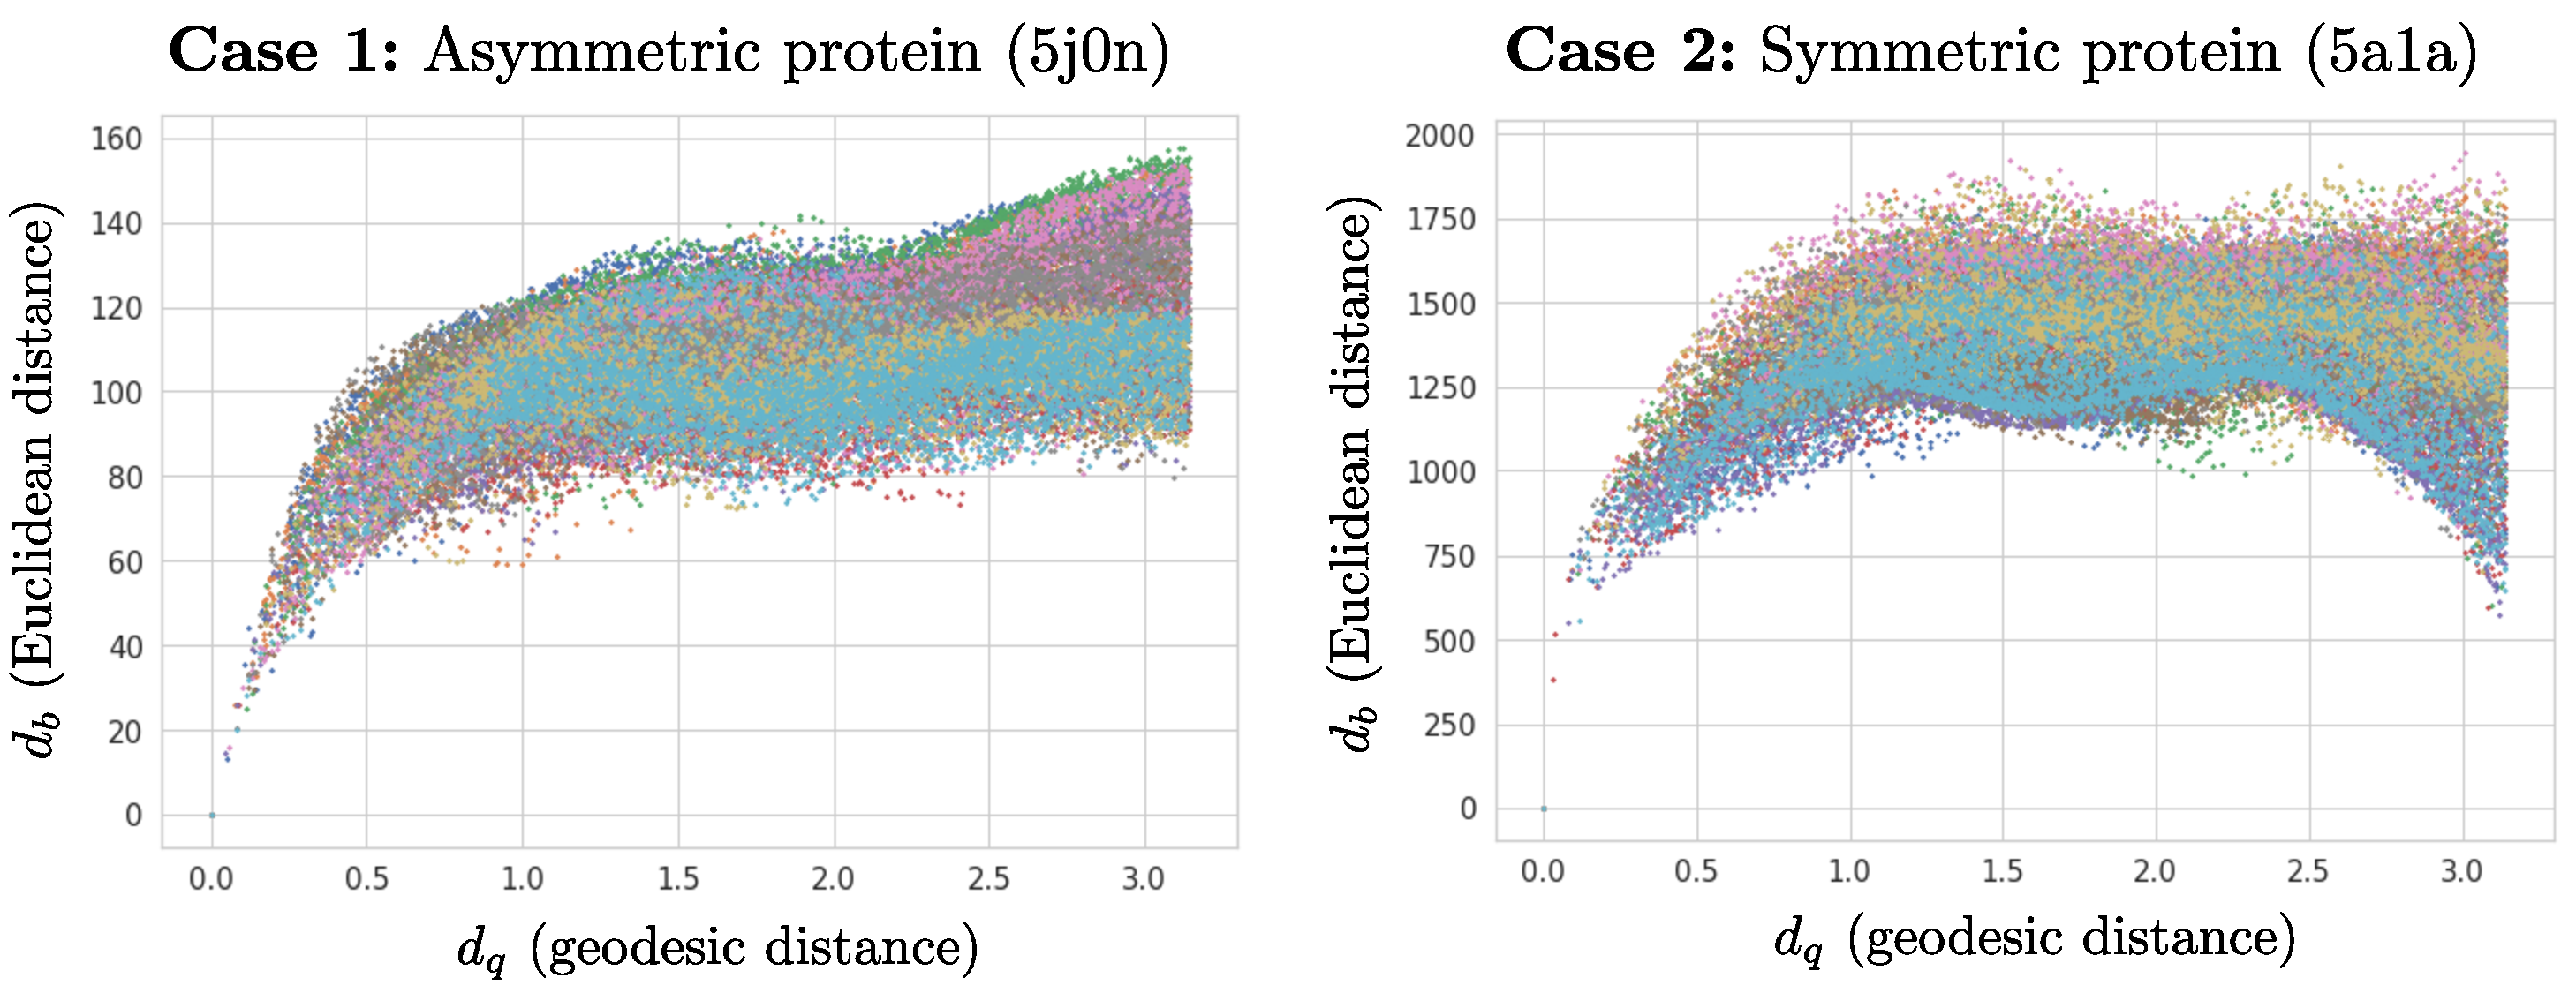
\includegraphics[width=\textwidth]{EuclideanDistance_NonRobust.pdf}
    \caption{Plotting the Euclidean distance between two projections versus their actual relative orientation (measured by the geodesic distance) for \textbf{(left)} the asymmetric protein (5j0n) dataset, and \textbf{(right)} the symmetric protein (5a1a) dataset. }
    \label{fig:euclidean-not-robust}
\end{figure}
%----

% -------------------------------
\subsubsection{Learning $\widehat{d}_b$ with a Siamese Neural Network}

As previously discussed, we make the choice to \textit{learn} a good approximation $\widehat{d}$ on a synthetic training dataset $\big\{ \mathbf{b}^{*p}, q^*_p\big\}_{p=1}^{N_t}$ through
%---
\begin{equation}
    \label{eq:metric-learning-siamese}
    \widehat{d}_b=\argmin{d_b}\sum_{i,j} \big|d_b\big(\mathbf{b}^{*i},\mathbf{b}^{*j}\big) - d_q\big(q^*_i,q^*_j\big) \big|^2,
\end{equation}
% ---
with $d_q$ defined in~\eqref{eq:geodesic distance}, and where $N_t$ indicates the number of projection-orientation pairs in the training dataset. More precisely, we parametrize the distance function $d_b$ in~\eqref{eq:metric-learning-siamese} as a Siamese neural network (SiameseNN)~\cite{chopra2005learning}, and resort to learning its weights $w$, as illustrated in Figure~\ref{fig:siamese-schematic}.

SiameseNNs, also termed ``twin networks'', are commonly used in the field of deep metric learning to learn similarity functions~\cite{yi2014deep}. They are usually constituted of two sister neural networks that work in tandem and share the exact same architecture and weights.  Their role (once trained) is to extract the projection features that are the most relevant to predict the relative orientation between two projections. The weights $w$ of the two sister networks are progressively learned by 1) comparing the difference of their projection feature vectors to the magnitude of the corresponding relative orientations, and 2) back-propagating this error (via the derivative chain rule) to the weights.

%---
\begin{figure}[t!]
    \centering
   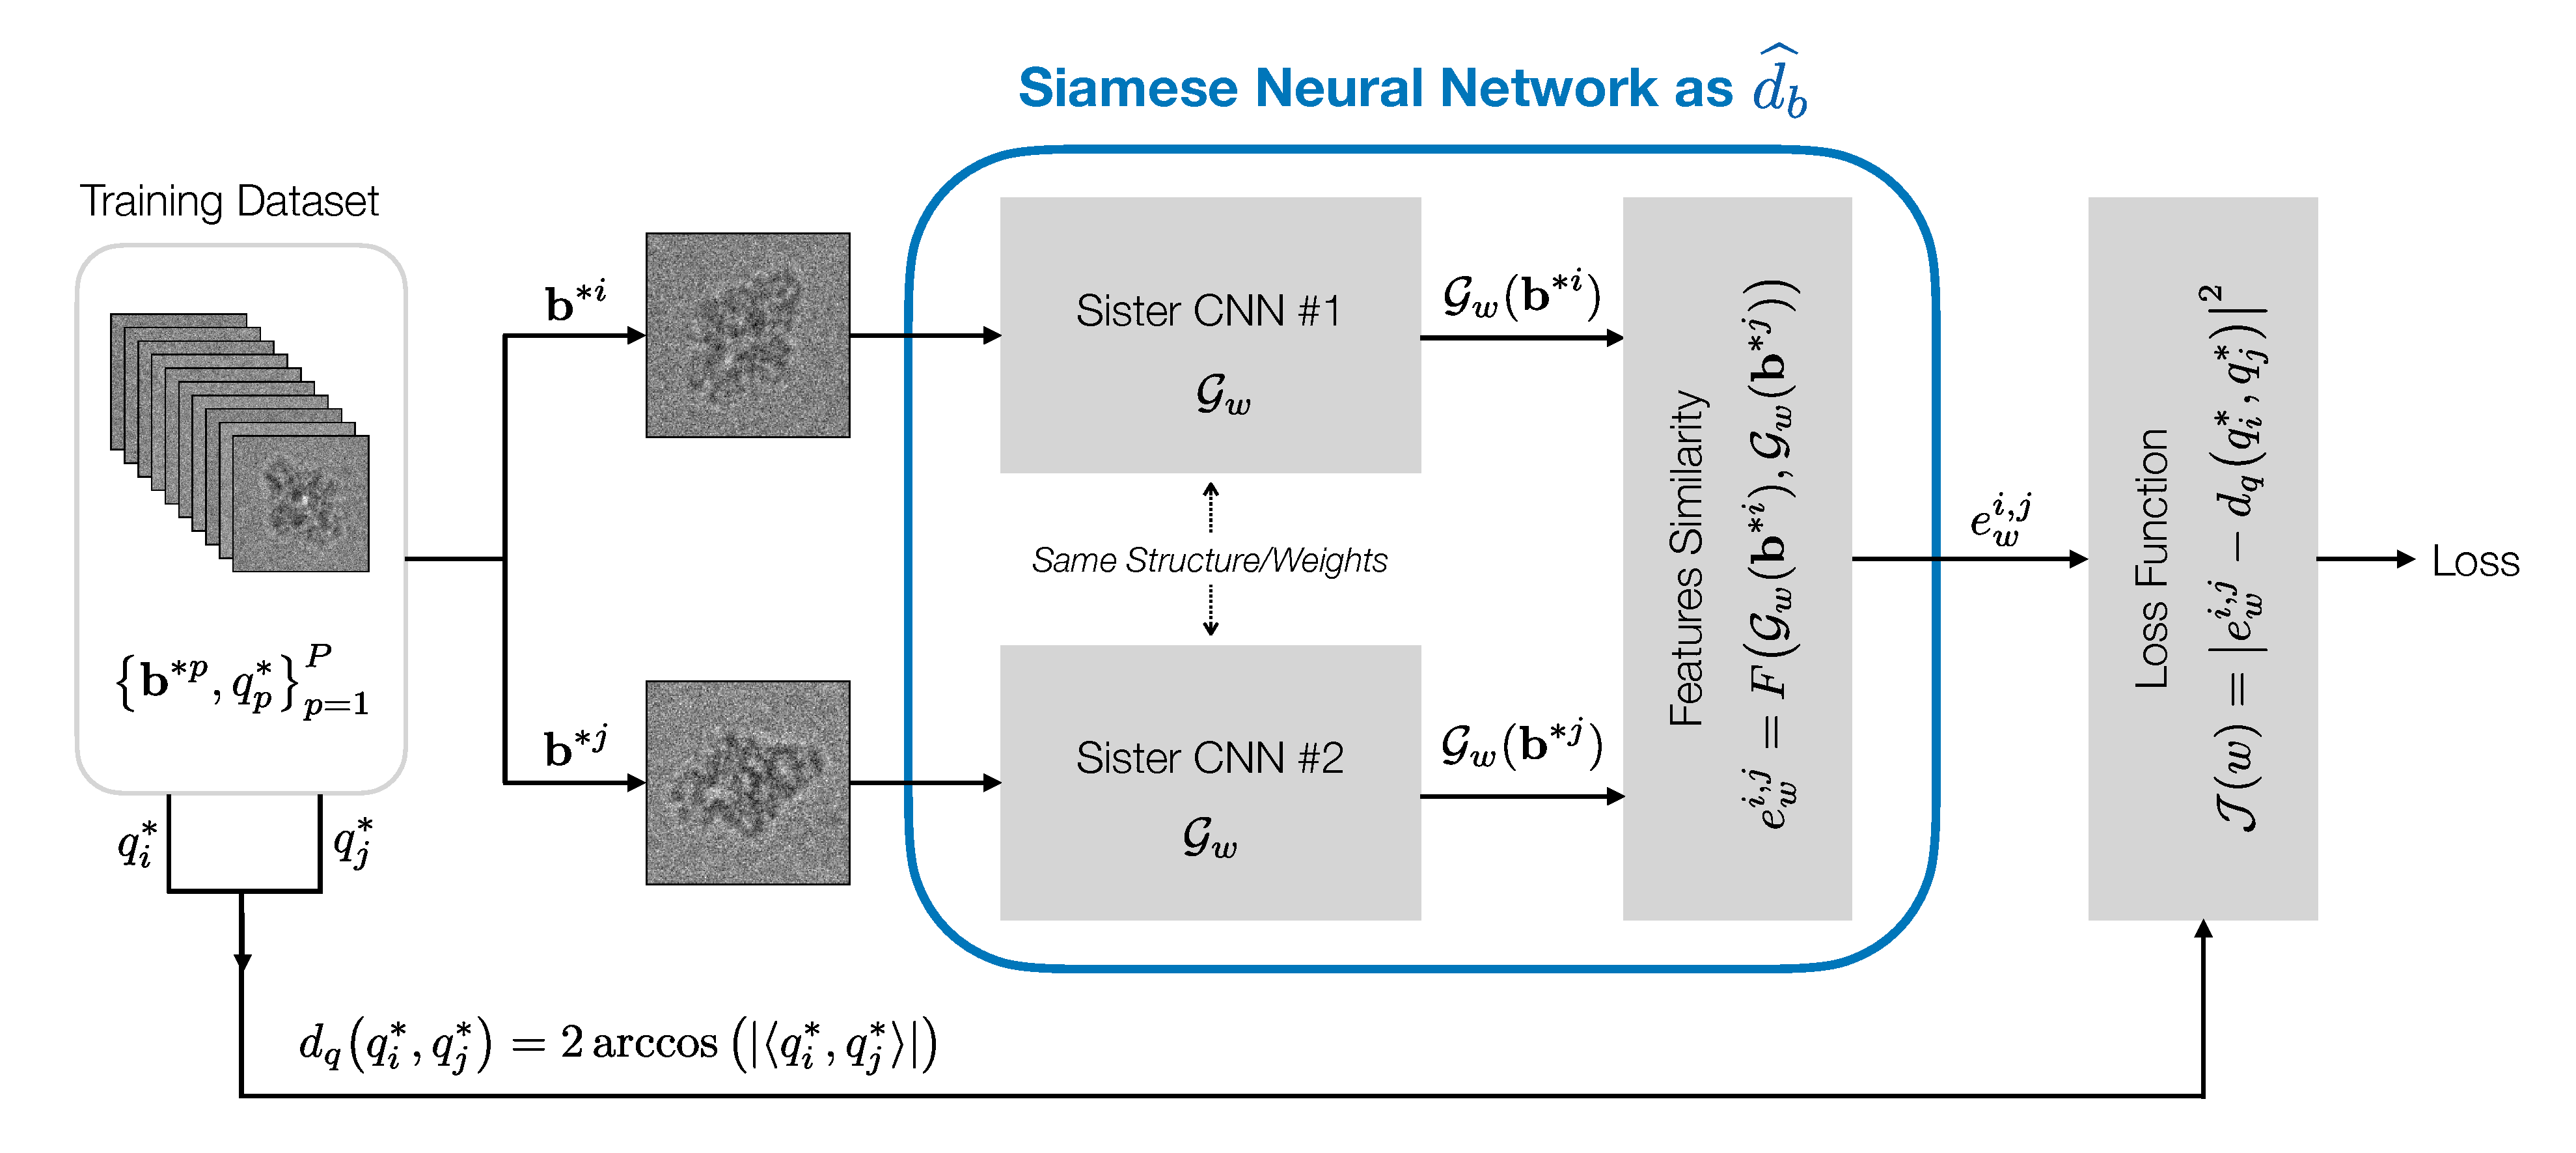
\includegraphics[width=\textwidth]{siameseNN-schematic.pdf}
    \caption{Training a Siamese neural network (SiameseNN) to become a faithful predictor of the relative orientation between two input projections. In other words, we train the SiameseNN to serve as a projection distance $\widehat{d}_b$ that correctly approximates the orientation distance $d_q$. The training is performed with a synthetic dataset that contains thousands of projections with their associated orientation.}
    \label{fig:siamese-schematic}
\end{figure}
% ---

% ----------------------------------------------------
\subsubsection{Generating a Proper Training Dataset for the SiameseNN}
\label{sec:training-siamese}

The success of the SiameseNN as a faithful predictor of relative orientations eventually relies on our capacity to generate a synthetic training dataset that is both large and representative of SPA measurements. In other words, we need to create a training set whose data distribution is diverse enough to cover that of unseen projection datasets. The objective is for the SiameseNN to be able to handle projections acquired in all sorts of imaging conditions and originating from 3D volumes it has never been trained on.

We shall create such comprehensive training dataset by capitalizing on two favorable conditions. First, there exists a large publicly-available database of deposited atomic models of proteins, which gives us access to thousands of different 3D ground truths. Then, we shall take advantage of our ability to model the cryo-EM imaging procedure to generate, from these ground truths, a synthetic dataset that contains a massive amount of realistic projections whose orientations are, by definition, all known.

Note that an interesting aspect of SiameseNNs for the present application is that they intrinsically predict the \textit{relationship} between objects. Hence, a well-trained SiameseNN could be relatively robust to the change of volumes. In the same line of thought, our SiameseNN will likely benefit from the profound structural similarity shared by proteins---after all, they all derived from just the same 21 amino acids.


% ----
\begin{figure}[t!]
    \centering
    \begin{subfigure}[t]{0.4\textwidth}
        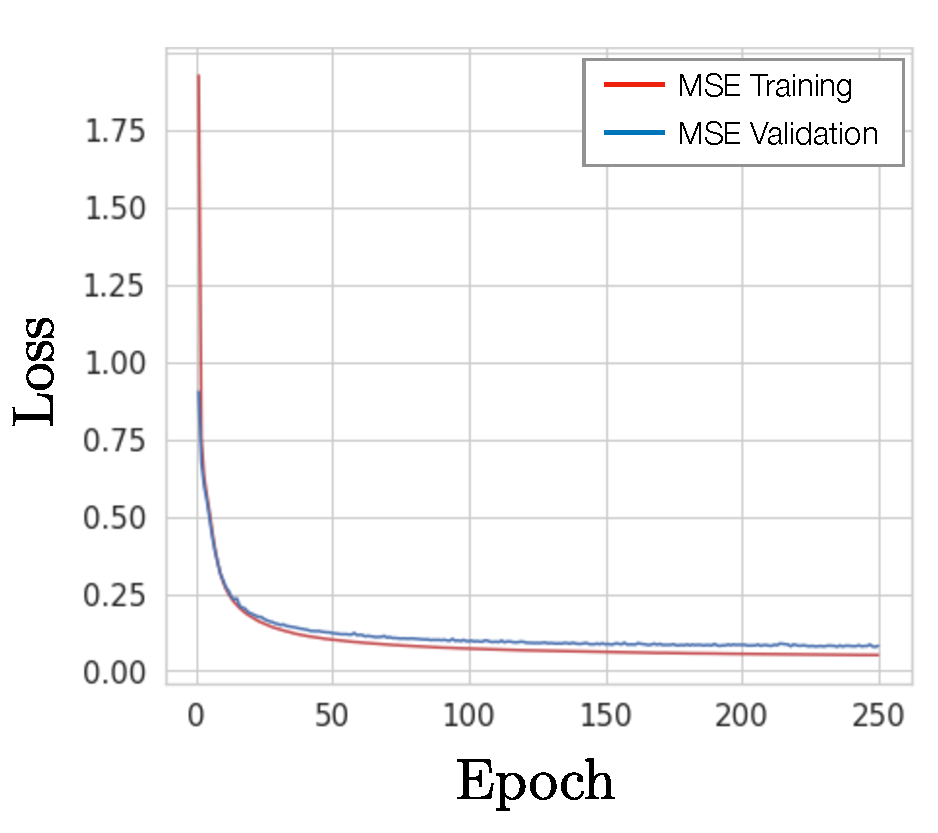
\includegraphics[width=0.98\textwidth]{TrainingSiamese_LossAssymetric.pdf}
        \caption{Training losses of the SiameseNN on the asymmetric protein (5j0n) training and validation datasets.}
        \label{fig:losses-siamese-assym}
    \end{subfigure} \quad \quad
    %
    \begin{subfigure}[t]{0.4\textwidth}
        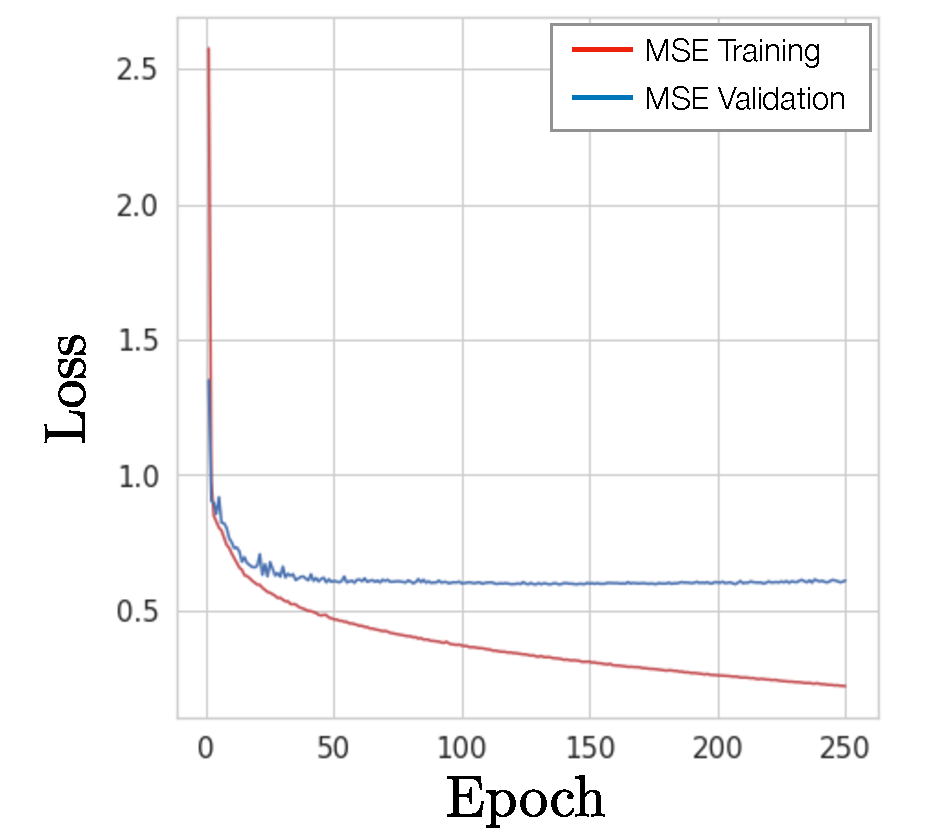
\includegraphics[width=0.98\textwidth]{TrainingSiamese_LossSymetric.pdf}
        \caption{Training losses of the SiameseNN on the symmetric protein (5a1a) training and validation datasets.}
        \label{fig:losses-siamese-sym}
    \end{subfigure} \vspace{0.45cm}

    %
    \begin{subfigure}[t]{0.4\textwidth}
        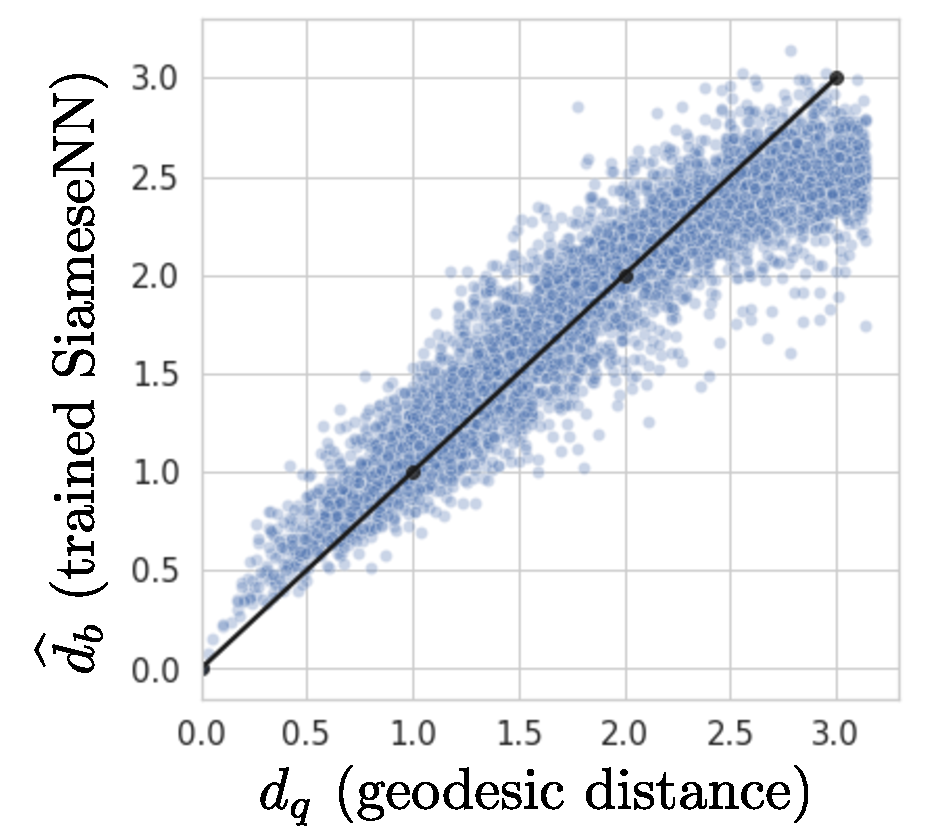
\includegraphics[width=0.98\textwidth]{TrainingSiamese_PlotAssymetric.pdf}
        \caption{Relative orientations predicted by the trained SiameseNN from projections in the asymmetric protein (5j0n) testing dataset. }
        \label{fig:learned-distance-siamese}
    \end{subfigure} \vspace{0.35cm}
    \caption{Training results for the SiameseNN.}
    \label{fig:losses-siamese}
\end{figure}
% ---


% ----------------------------------------------------
\subsubsection{Preliminary Training Results}

We present here a preliminary evaluation of the ability of SiameseNNs to learn a projection distance $\widehat{d}_b$ that correctly approximates the orientation distance $d_q$.

SiameseNNs come with a variety of more or less powerful architectures. At the current stage of development, we work with a simple one. Our SiameseNN is composed of two convolutional neural networks (CNNs) with shared weights. Their output features vectors are compared through an Eulidean distance, \textit{i.e.}, $F(\mathbf{x},\mathbf{y})=\lVert \mathbf{x}-\mathbf{y}\rVert_2$ in Figure~\ref{fig:siamese-schematic}. The detailed architecture of this SiameseNN is given in Figure~\ref{fig:app-SiameseNN-architecture} in Appendix X.

For each protein, we train the SiameseNN on its training dataset for 250 epochs ($\sim$10 hours) using an Adam optimizer~\cite{kingma2014adam}, a learning rate of $10^{-3}$, and a batch size of 256 projections. The evolution of the training and validation losses are presented in Figure~\ref{fig:losses-siamese-assym} for the asymmetric protein (5j0n), and in Figure~\ref{fig:losses-siamese-sym} for the symmetric one (5a1a). The results demonstrate that the SiameseNN succeeds at learning a proxy distance for the asymmetric protein dataset, as convergence is reached in about 50 epochs ($\sim$ 2 hours).

However, the current SiameseNN architecture fails at learning the distance for the dataset 5a1a, which is very likely due to the symmetry of the $\beta$-galactosidase protein. Indeed, its synthetic dataset contains pairs of projections that share the same $d_b$, yet differ in their $d_q$. This simply advocates for the restriction to non-overlapping areas on $\SOThree$ when sampling the orientations used to generate the SiameseNN training dataset. The latter would then only contain projection pairs with a linear $(d_q,d_b)$ relationship, which should ensure a successful training of the network. For the rest of the experiments, we use the asymmetric protein (5j0n) dataset.

We then feed to the trained SiameseNN $1,000$ pairs of projections randomly selected from the 5j0n testing dataset, and report the $(d_q,\widehat{d}_b)$ relationship of each pair in Figure~\ref{fig:learned-distance-siamese}. These results confirm that, for this protein at least, the SiameseNN is able to predict the orientation distance $d_q$ using only the projections as inputs. Moreover, it clearly outperforms the Euclidean distance at doing so. These preliminary results are encouraging, as much has yet to be gained from improving upon the rather primitive SiameseNN architecture we currently use.

\subsection{Orientation Recovery}
\label{sec:orientation-recovery}

Equipped with an appropriately learned $\widehat{d}_b$, the objective is then to recover the unknown unit quaternions $\big\{q_p\big\}_{p=1}^P$ associated to the projections $\big\{\mathbf{b}^p\big\}_{p=1}^P$ in any given dataset.

% ----------------------------------------------------
\subsubsection{Minimization Scheme}

We propose to start this process by computing of a great number of pairwise projection distances $\big\{\widehat{d}_b\big(\mathbf{b}^i,\mathbf{b}^j\big)\big\}_{i,j=1}^{P}$ through $\widehat{d}_b$. Then, our postulate is that we can recover the orientations from theses distances by solving
%---
\begin{equation}
    \label{eq:global-min-problem}
    \big\{\widehat{q}_p\big\}_{p=1}^P=\argmin{q_i\in\mathbb{U}}\sum_{i,j} \big|\widehat{d}_b\big(\mathbf{b}^i,\mathbf{b}^j\big) - d_q\big(q_i,q_j\big) \big|^2,
\end{equation}
% ---
as is illustrated in Figure~\ref{fig:overview-pipeline}.

In practice, one cannot possibly evaluate~\eqref{eq:global-min-problem} for every pair of orientations $\big\{q_i,q_j\big\}_{i,j=1}^P$ given the extremely large size of SPA datasets, with $P$ typically in the order of dozens of thousands. Hence, we need to partially sample the projection dataset. We experimentally demonstrate in Section~\ref{subsec:5-6-3-sanity-check} that this does not affect the performance of our recovery scheme.

As previously discussed, we are not yet aware of any guarantee of convergence for~\eqref{eq:global-min-problem}. Similarly, we do not know of any theoretical characterization of the behaviour of~\eqref{eq:global-min-problem} in ill-posed conditions, such as when pairwise distances are misestimated, for instance. Hence, we rely for now on experimental demonstrations to 1) ensure feasibility, and 2) indicate where efforts need to be invested.

% ----
\begin{figure}[t]
    \centering
    \begin{subfigure}[b]{0.48\textwidth}
        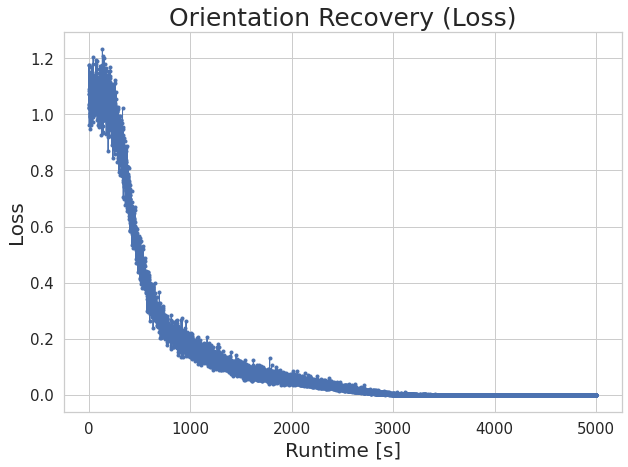
\includegraphics[width=\textwidth]{fig_perfectdistances_loss-symmetric.png}
        \caption{}
    \end{subfigure} \quad
    \begin{subfigure}[b]{0.48\textwidth}
    \centering
        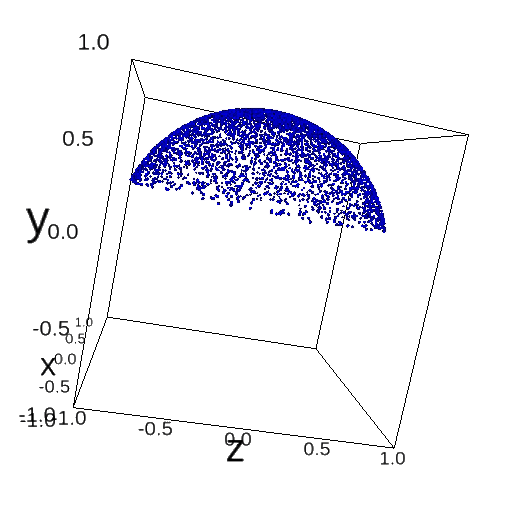
\includegraphics[width=0.8\textwidth]{fig-perfectdistances-coverage-symmetric.png}
        \caption{}
    \end{subfigure}
    \caption{Results of the orientation recovery scheme when using the perfect orientation distances for the asymmetric protein (5j0n). \textbf{(a)} Evolution of the loss of~\eqref{eq:global-min-problem} during minimization. \textbf{(b)} Coverage of $\SOThree$ after the orientation recovery from the perfect relative distances. }
    \label{fig:minim-loss-perfect-distances}
\end{figure}
% ---

% ----------------------------------------------------
\subsubsection{Feasibility Check: Recovery from the Exact Relative Distances}
\label{subsec:5-6-3-sanity-check}

Our first investigation is to verify that it is at all possible to recover the orientations through~\eqref{eq:global-min-problem} from their true relative distances (\textit{i.e.}, using $d_q$ and not a proxy $d_b$).

We use the $5,000$ projections from the asymmetric protein (5j0n) dataset. Out of the possible 25 mio possible pairs, we randomly select only $5,000$ of them and compute their geodesic distance through~\eqref{eq:geodesic distance}. We then minimize~\eqref{eq:global-min-problem} using the SGD Adam optimizer~\cite{kingma2014adam} for $30K$ steps ($\sim$1 hour) with a learning rate of $0.1$.

The results are given in Figure~\ref{fig:minim-loss-perfect-distances}. They confirm that it is possible to recover the orientations from their true relative distances, even though the embedding space is non-Euclidean. As previously discussed, this is not a straightforward result. The results also demonstrate that a large subsampling of the projection pairs does not affect the convergence of~\eqref{eq:global-min-problem}, which is in straight line with the observations made by numerous Euclidean-based dimensionality reduction works~\cite{belkin2003laplacian,kruskal1978multidimensional, maaten2008visualizing, mcinnes2018umap}.

% ----------------------------------------------------
\subsubsection{Robustness of Recovery to Additive Errors on the Relative Distances}
\label{subsec:5-6-4-robustness-to-errors}

We now go one step further and evaluate the behaviour of~\eqref{eq:global-min-problem} when the true relative distances are corrupted by  additive Gaussian noise.

The experimental conditions are the same than in the previous section, except that we add an error with increasing variance on the relative distances prior to the minimization. The results are presented in Figure~\ref{fig:recovery-noise-distances} (red curve).

% ----
\begin{figure}
    \centering
    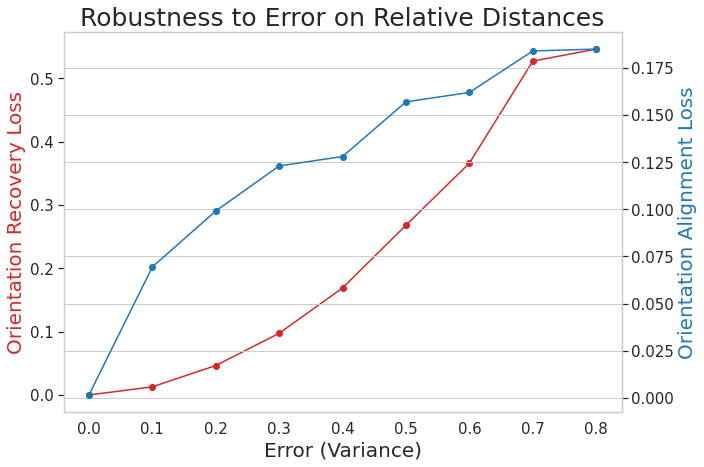
\includegraphics[width=0.75\textwidth]{fig-robustness-asymmetric.png}
    \caption{Results of the recovery scheme (red curve) and the alignment procedure (blue curve) when an increasing amount of errors is added to the true relative distances.}
    \label{fig:recovery-noise-distances}
\end{figure}
% ---

Before discussing the results, we remark that one cannot really quantify the performance of~\eqref{eq:global-min-problem} through its loss. Unfortunately, it is also not appropriate to directly compute the error between the recovered orientations $\big\{\widehat{q}_p\big\}_{p=1}^P$ and the true ones $\big\{q_p\big\}_{p=1}^P$. The reason is that the recovery of orientation through~\eqref{eq:global-min-problem} is up to a global rotation, \textit{i.e.}, any global rotation of the set of recovered orientations is as valid as any other. This is not a problem for the ultimate application of our scheme, but it complicates the quantitative evaluation of its performance in synthetic experiments. We circumvent this problem by 1) aligning the true and recovered orientation sets, and 2) computing their distance after alignment. The alignment is performed by searching for the orthogonal matrix (with determinant $\pm$ 1) $\mathbf{T}\in\mathbb{R}^4$  that minimizes
% ---
\begin{equation}
    \label{eq:alignement}
    \widehat{\mathbf{T}}=\argmin{\mathbf{T}\in\mathbb{R}^4}\sum_{i,j} \big|d_q\big(q_i,q_j\big)- d_q\big(\mathbf{T}\widehat{q}_i,\mathbf{T}\widehat{q}_j\big)\big|^2.
\end{equation}
% ---
For all variances, the distance after alignment is reported in Figure~\ref{fig:recovery-noise-distances} (blue curve).

These results demonstrate that the performance of the minimization scheme~\eqref{eq:global-min-problem} linearly depends on the quality of the relative distances, which advocates for a proper and extensive training of the SiameseNN in the next stages of development. Another interesting output of Figure~\ref{fig:recovery-noise-distances} is that it indicates that the error of the orientation recovery behaves as a monotonic function of its loss. Hence, it suggests that the loss can be used as a good indicator of its performance, which has obvious practical implications for our future works on real data.
